\documentclass[aspectratio=169,10pt]{beamer}
\usepackage[utf8]{inputenc}
\usepackage{amsmath, amssymb, bm, amsfonts}
\usepackage{booktabs}
\usepackage{listings}
\usepackage{graphicx}
\usepackage{tikz}
\usetikzlibrary{arrows.meta, positioning, calc, angles, quotes, shapes.geometric}

% ==============================================================================
% UNIVERSIDAD DE ANTIOQUIA (UdeA) BRANDING & PALETTE
% ==============================================================================
\definecolor{UdeAGreen}{HTML}{006241} % Institutional Dark Green
\definecolor{UdeAGold}{HTML}{D4AF37}  % Institutional Gold
\definecolor{Charcoal}{HTML}{2B2B2B}  % Text Charcoal
\definecolor{LightBg}{HTML}{F8F9FA}   % Slide Canvas Background
\definecolor{DarkSlate}{RGB}{15, 23, 42} % Dark Slate for Containers
\definecolor{AlertRed}{RGB}{220, 38, 38}

\setbeamercolor{palette primary}{bg=UdeAGreen, fg=white}
\setbeamercolor{palette secondary}{bg=UdeAGreen, fg=white}
\setbeamercolor{structure}{fg=UdeAGreen}
\setbeamercolor{background canvas}{bg=LightBg}
\setbeamercolor{text}{fg=Charcoal}

% --- Block Customization ---
\setbeamercolor{block title}{bg=UdeAGreen, fg=white}
\setbeamercolor{block body}{bg=white, fg=Charcoal}
\setbeamercolor{block title example}{bg=UdeAGold, fg=Charcoal}
\setbeamercolor{block body example}{bg=white, fg=Charcoal}
\setbeamercolor{block title alerted}{bg=AlertRed, fg=white}
\setbeamercolor{block body alerted}{bg=white, fg=Charcoal}

% --- Header/Footer Customization ---
\setbeamertemplate{headline}{}
\setbeamertemplate{footline}{%
    \leavevmode%
    \begin{beamercolorbox}[wd=\paperwidth,ht=2.5ex,dp=1.125ex,leftskip=.3cm,rightskip=.3cm]{palette primary}%
        \footnotesize Universidad de Antioquia -- Faculty of Engineering \hfill Astrodynamics 2026-2 \hfill \insertframenumber/\inserttotalframenumber%
    \end{beamercolorbox}%
}
\setbeamertemplate{navigation symbols}{}

\usetheme{Madrid}
\usefonttheme{professionalfonts}

\title[Pure RAAN Change Geometry]{\textbf{Non-Coplanar Orbital Maneuvers:}}
\subtitle{The Physics, Geometry, and Vector Mechanics of Pure RAAN (\texorpdfstring{$\Delta\Omega$}{Delta-Omega}) Transfers}
\author{Prof. Juan Francisco Puerta Ibarra}
\institute{Department of Aerospace Engineering --- Faculty of Engineering \\ Universidad de Antioquia (UdeA)}
\date{Semester 2026-2}
\titlegraphic{
\includegraphics[width=2.0cm]{Images/UdeA+simplificado+Negro_Smaller.png}}

\begin{document}

% ------------------------------------------------------------------------------
% SLIDE 1: TITLE SLIDE
% ------------------------------------------------------------------------------
\begin{frame}[plain]
    \titlepage
\end{frame}

% ------------------------------------------------------------------------------
% SLIDE 2: THE OPERATIONAL ANOMALY
% ------------------------------------------------------------------------------
\begin{frame}{The Operational Anomaly: The "Apex Firing" Trap}
    \begin{columns}[t]
        \begin{column}{0.54\textwidth}
            \begin{alertblock}{The Problem in Flight Operations}
                \footnotesize
                Students and mission designers often calculate the theoretical scalar impulse requirement:
                \vspace{-0.15cm}
                $$\Delta V_\Omega = 2 v_c \sin(i)\sin\left(\frac{\Delta\Omega}{2}\right)$$
                \vspace{0.25cm}
                and command an impulsive burn at the orbital apex ($u = \theta + \omega = 90^\circ$).
            \end{alertblock}
            \vspace{0.08cm}
            \footnotesize
            \textbf{The Operational Consequence:}
            \begin{itemize}\setlength{\itemsep}{2pt}
                \item The line of nodes shifts by $\Delta\Omega$ as commanded.
                \item \textbf{Unintended Inclination Leak:} The final inclination increases ($i_{\text{final}} > i_{\text{initial}}$)!
                \item The orbit becomes eccentric if fired purely along the normal axis ($\hat{\mathbf{N}}$).
            \end{itemize}
        \end{column}
        
        \begin{column}{0.44\textwidth}
            \begin{block}{Why Does This Occur?}
                \footnotesize
                \begin{enumerate}\setlength{\itemsep}{4pt}
                    \item \textbf{Infinitesimal vs. Finite:} Gauss's Variational Equation ($di/dt = 0$ at $u = 90^\circ$) applies strictly to \textit{infinitesimal continuous thrust}, not finite impulsive burns.
                    \item \textbf{Plane Intersection Geometry:} Two orbits with identical inclination $i$ separated by $\Delta\Omega$ \textbf{do not intersect at $u = 90^\circ$}!
                \end{enumerate}
            \end{block}
        \end{column}
    \end{columns}
\end{frame}

% ------------------------------------------------------------------------------
% SLIDE 3: FOUNDATIONAL COORDINATES: THE ARGUMENT OF LATITUDE (u)
% ------------------------------------------------------------------------------
\begin{frame}{Foundational Coordinates: The Argument of Latitude (\texorpdfstring{$u$}{u})}
    \begin{columns}[t]
        \begin{column}{0.50\textwidth}
            \begin{block}{Definition: The Composite Angle $u$}
                \footnotesize
                The \textbf{Argument of Latitude} $u$ defines the angular position of a spacecraft measured along the orbital plane from the \textbf{Ascending Node}:
                \begin{equation}
                    u = \omega + \theta
                \end{equation}
                where $\omega$ is the argument of periapsis and $\theta$ is the true anomaly.
                
                \vspace{0.05cm}
                In vector notation, using the node vector $\mathbf{n} = \mathbf{\hat{K}} \times \mathbf{h}$:
                \begin{equation}
                    \cos u = \frac{\mathbf{n} \cdot \mathbf{r}}{\|\mathbf{n}\| \|\mathbf{r}\|} \quad (u > 180^\circ \text{ if } r_z < 0)
                \end{equation}
            \end{block}

            \begin{exampleblock}{Spherical Latitude Mapping ($\phi$)}
                \footnotesize
                The instantaneous geocentric latitude $\phi$ satisfies:
                \begin{equation}
                    \sin \phi = \sin i \sin u
                \end{equation}
            \end{exampleblock}
        \end{column}

        \begin{column}{0.48\textwidth}
            \begin{alertblock}{Why $u$ is Indispensable for Circular Orbits}
                \footnotesize
                \begin{itemize}\setlength{\itemsep}{2pt}
                    \item In circular orbits ($e = 0$), the periapsis is \textbf{undefined} (no unique point of closest approach).
                    \item Consequently, $\omega$ and $\theta$ suffer from a severe $0/0$ \textbf{mathematical singularity}.
                    \item The composite angle $u = \omega + \theta$ bypasses this singularity completely, providing a smooth, non-singular coordinate directly referenced to the equator!
                \end{itemize}
            \end{alertblock}

            \begin{block}{Four Landmark Points Along Orbit}
                \scriptsize
                \begin{itemize}\setlength{\itemsep}{1pt}
                    \item $u = 0^\circ$: Ascending Node ($\phi = 0^\circ$, Northbound)
                    \item $\mathbf{u = 90^\circ}$: \textbf{Orbital Apex} ($\phi = +i$, Peak Latitude)
                    \item $u = 180^\circ$: Descending Node ($\phi = 0^\circ$, Southbound)
                    \item $u = 270^\circ$: Orbital Antiapex ($\phi = -i$, Trough)
                \end{itemize}
            \end{block}
        \end{column}
    \end{columns}
\end{frame}

% ------------------------------------------------------------------------------
% SLIDE 4: ORBITAL PLANE GEOMETRY: VISUALIZING u IN 3D (ERROR-FREE & PINNED)
% ------------------------------------------------------------------------------
\begin{frame}{Orbital Plane Geometry: Visualizing the Angle \texorpdfstring{$u = \omega + \theta$}{u = omega + theta}}
    \begin{columns}[c]
        \begin{column}{0.54\textwidth}
            \centering
            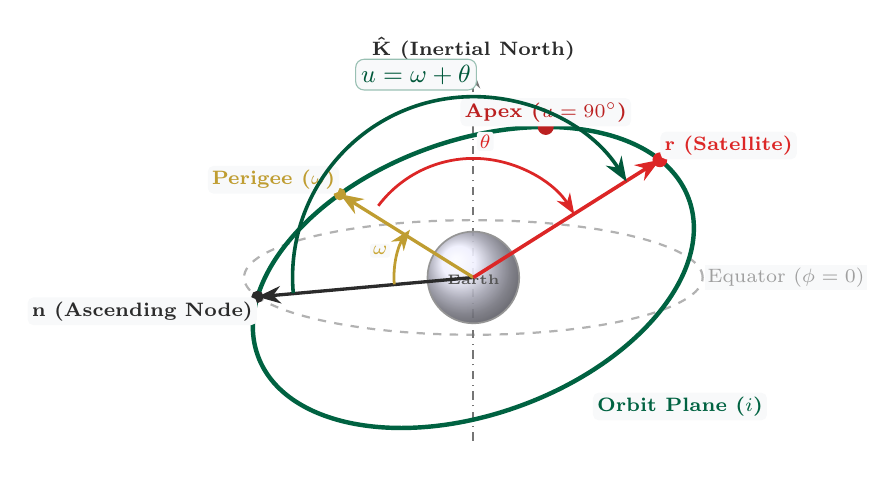
\begin{tikzpicture}[scale=1.12, >=Stealth]
                % 1. Celestial Equator Plane (Gray Dashed Ellipse)
                \draw[color=gray!60, dashed, line width=0.8pt] (0,0) ellipse (2.60cm and 0.65cm);
                \node[right, font=\scriptsize, color=gray!75, fill=LightBg, inner sep=1pt] at (2.62, 0) {Equator ($\phi = 0$)};

                % 2. Polar Axis (Z-axis / Inertial North)
                \draw[->, color=Charcoal!65, dashdotted, line width=0.8pt] (0,-1.85) -- (0,2.35) 
                    node[above, font=\scriptsize\bfseries, color=Charcoal] {$\mathbf{\hat{K}}$ (Inertial North)};

                % 3. Inclined Orbit Plane (Solid Green Ellipse tilted by i)
                \draw[rotate=20, color=UdeAGreen, line width=1.6pt] (0,0) ellipse (2.60cm and 1.55cm);
                \node[below right, font=\scriptsize\bfseries, color=UdeAGreen, fill=LightBg, rounded corners=2pt, inner sep=1.5pt] 
                    at (1.35, -1.30) {Orbit Plane ($i$)};

                % 4. Earth Sphere (Clean Soft Shading in Center)
                \shade[ball color=LightBg!75!blue!30, opacity=0.9] (0,0) circle (0.52cm);
                \draw[color=Charcoal!50, line width=0.6pt] (0,0) circle (0.52cm);
                \node[font=\tiny\bfseries, color=Charcoal!80] at (0, -0.02) {Earth};

                % -------------------------------------------------------------
                % MATHEMATICALLY CONSTRAINED POINTS (INSIDE SCOPE, ZERO PARSER CONFLICT)
                % -------------------------------------------------------------
                \begin{scope}[rotate=20]
                    \coordinate (Node) at ({2.60*cos(156)}, {1.55*sin(156)});
                    \coordinate (Perigee) at ({2.60*cos(115)}, {1.55*sin(115)});
                    \coordinate (Apex) at ({2.60*cos(58.6)}, {1.55*sin(58.6)});
                    \coordinate (Sat) at ({2.60*cos(20)}, {1.55*sin(20)});
                \end{scope}

                % 5. Line of Nodes Vector (n)
                \draw[->, color=Charcoal, line width=1.2pt] (0,0) -- (Node);
                \filldraw[color=Charcoal] (Node) circle (1.8pt);
                \node[below left, font=\scriptsize\bfseries, color=Charcoal, fill=LightBg, rounded corners=2pt, inner sep=1.5pt] 
                    at (Node) {$\mathbf{n}$ (Ascending Node)};

                % 6. Perigee Direction Vector
                \draw[->, color=UdeAGold!90!black, line width=1.2pt] (0,0) -- (Perigee);
                \filldraw[color=UdeAGold!90!black] (Perigee) circle (1.8pt);
                \node[above left, font=\scriptsize\bfseries, color=UdeAGold!90!black, fill=LightBg, rounded corners=2pt, inner sep=1.5pt] 
                    at (Perigee) {Perigee ($\omega$)};

                % 7. Satellite Position Vector (r)
                \draw[->, color=AlertRed, line width=1.3pt] (0,0) -- (Sat);
                \filldraw[color=AlertRed] (Sat) circle (2.2pt);
                \node[above right, font=\scriptsize\bfseries, color=AlertRed, fill=LightBg, rounded corners=2pt, inner sep=1.5pt] 
                    at (Sat) {$\mathbf{r}$ (Satellite)};

                % 8. Orbital Apex (PINNED EXACTLY ONTO THE GREEN ORBIT)
                \filldraw[color=AlertRed!85!black] (Apex) circle (2.4pt);
                \node[above, font=\scriptsize\bfseries, color=AlertRed!85!black, fill=LightBg, rounded corners=2pt, inner sep=1.5pt] 
                    at (Apex) {Apex ($u=90^\circ$)};

                % -------------------------------------------------------------
                % CONCENTRIC ANGLE ARCS
                % -------------------------------------------------------------
                % Inner Arc 1: Argument of Perigee (\omega) [r = 0.90 cm]
                \draw[->, color=UdeAGold!90!black, line width=1.0pt] (185:0.90) arc (185:143:0.90);
                \node[font=\scriptsize\bfseries, color=UdeAGold!95!black, fill=LightBg, rounded corners=1pt, inner sep=1pt] 
                    at (164:1.10) {$\omega$};

                % Middle Arc 2: True Anomaly (\theta) [r = 1.35 cm]
                \draw[->, color=AlertRed, line width=1.0pt] (143:1.35) arc (143:32:1.35);
                \node[font=\scriptsize\bfseries, color=AlertRed, fill=LightBg, rounded corners=1pt, inner sep=1pt] 
                    at (85:1.55) {$\theta$};

                % Outer Arc 3: Composite Argument of Latitude (u = \omega + \theta) [r = 2.05 cm]
                \draw[->, color=UdeAGreen!90!black, line width=1.3pt] (185:2.05) arc (185:32:2.05);
                \node[font=\small\bfseries, color=UdeAGreen!90!black, fill=LightBg, rounded corners=3pt, draw=UdeAGreen!40, inner sep=2pt] 
                    at (-0.65, 2.30) {$u = \omega + \theta$};
            \end{tikzpicture}
        \end{column}

        \begin{column}{0.44\textwidth}
            \begin{block}{Spatial Takeaways: The Role of $u$}
                \footnotesize
                \begin{itemize}\setlength{\itemsep}{4pt}
                    \item $\mathbf{n}$ defines the zero-reference angle on the orbital plane ($u = 0^\circ$).
                    \item The satellite climbs in latitude until it reaches the \textbf{Orbital Apex} at $u = 90^\circ$ ($\phi = +i$).
                    \item It then descends through the Descending Node ($u = 180^\circ$, $\phi = 0^\circ$).
                    \item \textbf{Targeting Connection:} Plane changes that rotate the line of nodes ($\Delta\Omega$) must be timed in terms of $u$, because the node is the equatorial anchor!
                \end{itemize}
            \end{block}
        \end{column}
    \end{columns}
\end{frame}

% ------------------------------------------------------------------------------
% SLIDE 5: GAUSS VARIATIONAL EQUATIONS (WHY THEORY POINTS TO APEX)
% ------------------------------------------------------------------------------
\begin{frame}{Gauss's Variational Equations: Why Theory Points to the Apex}
    \begin{block}{Gauss's Variational Equations for Out-of-Plane Acceleration ($f_h$)}
        \footnotesize
        $$\frac{di}{dt} = \frac{r \cos u}{h} f_h, \qquad \frac{d\Omega}{dt} = \frac{r \sin u}{h \sin i} f_h$$
    \end{block}
    \vspace{0.1cm}
    \begin{columns}[t]
        \begin{column}{0.48\textwidth}
            \begin{block}{The Theoretical Allure of $u = 90^\circ$}
                \scriptsize
                \begin{itemize}\setlength{\itemsep}{3pt}
                    \item $\cos(90^\circ) = 0 \implies \frac{di}{dt} = 0$ (zero instantaneous inclination change).
                    \item $\sin(90^\circ) = 1 \implies \frac{d\Omega}{dt} = \text{maximum}$ (maximum nodal precession rate).
                    \item Setting $u = 90^\circ$ seems mathematically optimal to rotate $\Omega$ without disturbing $i$.
                \end{itemize}
            \end{block}
        \end{column}
        
        \begin{column}{0.48\textwidth}
            \begin{alertblock}{The Core Limitation of Gauss's Law}
                \scriptsize
                \begin{itemize}\setlength{\itemsep}{3pt}
                    \item Gauss's equations are \textbf{first-order differential rates} derived for continuous, infinitesimal thrust ($f_h \to 0$).
                    \item They represent the instantaneous rate of change of osculating elements at a single point in time.
                    \item An impulsive maneuver applies a \textbf{finite $\Delta\mathbf{V}$ instantaneously}, violating the differential continuum assumption!
                \end{itemize}
            \end{alertblock}
        \end{column}
    \end{columns}
\end{frame}

% ------------------------------------------------------------------------------
% SLIDE 6: THE PHYSICS OF THE GAUSS APEX TRAP
% ------------------------------------------------------------------------------
\begin{frame}{The Physics of the Gauss Apex Trap: Rates vs. Finite Geometry}
    \begin{columns}[t]
        \begin{column}{0.50\textwidth}
            \begin{block}{Why the Apex Trap Occurs}
                \scriptsize
                \begin{itemize}\setlength{\itemsep}{3pt}
                    \item \textbf{Forced Conic Boundary Condition:} A spacecraft executing an impulsive burn $\Delta\mathbf{V}$ at position $\mathbf{r}_0$ forces the post-burn orbit to pass through $\mathbf{r}_0$.
                    \item At $u_1 = 90^\circ$, Orbit 1 reaches its maximum northern latitude: $\phi = i$.
                    \item Because Orbit 2 is shifted eastward by $\Delta\Omega$, \textbf{its apex is also shifted eastward}.
                    \item Thus, the burn point $\mathbf{r}_0$ is \textbf{not} the apex of Orbit 2!
                \end{itemize}
            \end{block}
        \end{column}
        
        \begin{column}{0.48\textwidth}
            \begin{alertblock}{The Inclination Overshoot ($\Delta i > 0$)}
                \scriptsize
                \begin{itemize}\setlength{\itemsep}{3pt}
                    \item If Orbit 2 has latitude $\phi = i$ at a location that is \textit{not} its apex, the orbit must continue climbing down-track.
                    \item The true peak latitude of Orbit 2 is higher than $i$:
                    $$\sin(i_{\text{achieved}}) = \frac{\sin i}{\cos(\delta u)} > \sin i \implies \mathbf{i_{\text{achieved}} > i}$$
                    \item An apex burn guarantees an \textbf{inclination leak} ($\Delta i > 0$).
                \end{itemize}
            \end{alertblock}
        \end{column}
    \end{columns}
    \vspace{0.1cm}
    \begin{exampleblock}{The Astrodynamic Resolution}
        \scriptsize
        Gauss tells us where the \textit{instantaneous rate} $\frac{di}{dt}$ vanishes for continuous acceleration. But for a finite impulsive burn, the maneuver must be executed at the \textbf{true geometric intersection of the two planes}: $u_{\text{burn}} = 90^\circ + \delta u$.
    \end{exampleblock}
\end{frame}

% ------------------------------------------------------------------------------
% SLIDE 7: SCHEMATIC ANATOMY OF THE APEX TRAP (ENLARGED & RESIZED)
% ------------------------------------------------------------------------------
\begin{frame}{Schematic Anatomy: Why the New Peak Must Rise Higher}
    \centering
    \vspace{-0.15cm}
    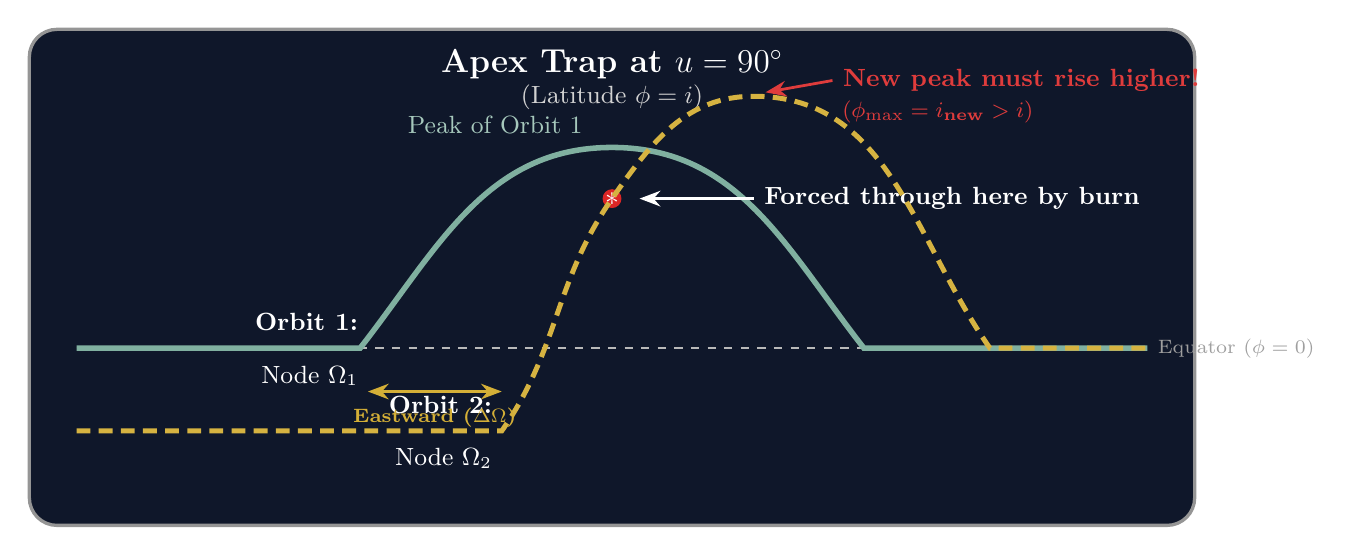
\begin{tikzpicture}[scale=1.0, >=Stealth]
        % Enlarged Dark slate background container filling the 16:9 widescreen frame
        \draw[fill=DarkSlate, rounded corners=10pt, draw=Charcoal!50, line width=1.2pt] 
            (-7.4, -3.1) rectangle (7.4, 3.2);
        
        % Equator Baseline Reference Line
        \draw[dashed, color=gray!55, line width=0.8pt] 
            (-6.8, -0.85) -- (6.8, -0.85) 
            node[right, font=\scriptsize, color=gray!75] {Equator ($\phi = 0$)};
        
        % Top Titles Inside Container
        \node[above, font=\large\bfseries, color=white] at (0, 2.45) {Apex Trap at $u = 90^\circ$};
        \node[above, font=\small, color=gray!35] at (0, 2.05) {(Latitude $\phi = i$)};
        
        % Orbit 1 (Solid Teal / Green Trajectory)
        \draw[color=UdeAGreen!50!white, line width=2.0pt] 
            (-6.8, -0.85) -- (-3.2, -0.85)
            to[out=52, in=180] (0, 1.70)
            to[out=0, in=128] (3.2, -0.85) -- (6.8, -0.85);
            
        % Orbit 1 Node Labels
        \node[above left, font=\small\bfseries, color=white] at (-3.1, -0.75) {Orbit 1:};
        \node[below left, font=\small, color=white] at (-3.1, -0.95) {Node $\Omega_1$};
        \node[above left, font=\small, color=UdeAGreen!35!white] at (-0.25, 1.75) {Peak of Orbit 1};
        
        % Burn Point Marker (*) at Apex Meridian
        \filldraw[color=AlertRed] (0, 1.05) circle (3.2pt);
        \node[font=\bfseries\normalsize, color=white] at (0, 1.05) {$*$};
        
        % Callout Arrow: Forced Through Here by Burn
        \draw[<-, color=white, line width=1.0pt] (0.35, 1.05) -- (1.8, 1.05) 
            node[right, font=\small\bfseries, color=white] {Forced through here by burn};
        
        % Orbit 2 (Dashed Gold Trajectory - Shifted Eastward)
        \draw[color=UdeAGold!95!white, line width=1.8pt, dash pattern=on 5pt off 3pt] 
            (-6.8, -1.90) -- (-1.4, -1.90)
            to[out=55, in=235] (0, 1.05)
            to[out=55, in=180] (1.8, 2.35)
            to[out=0, in=125] (4.8, -0.85) -- (6.8, -0.85);
            
        % Orbit 2 Node Labels
        \node[above left, font=\small\bfseries, color=white] at (-1.4, -1.80) {Orbit 2:};
        \node[below left, font=\small, color=white] at (-1.4, -2.00) {Node $\Omega_2$};
        
        % Eastward Nodal Shift Arrow (Positioned cleanly with zero overlap)
        \draw[<->, color=UdeAGold, line width=1.0pt] (-3.1, -1.40) -- (-1.4, -1.40) 
            node[midway, below=2pt, font=\scriptsize\bfseries, color=UdeAGold] {Eastward ($\Delta\Omega$)};
        
        % Orbit 2 Peak Overshoot Callout
        \draw[<-, color=AlertRed!90!white, line width=1.0pt] (1.95, 2.40) -- (2.8, 2.55) 
            node[right, font=\small\bfseries, color=AlertRed!90!white] {New peak must rise higher!};
        \node[right, font=\footnotesize\bfseries, color=AlertRed!90!white] at (2.8, 2.15) 
            {$(\phi_{\max} = i_{\text{new}} > i)$};
    \end{tikzpicture}
\end{frame}

% ------------------------------------------------------------------------------
% SLIDE 8: DIAGRAM - 3D CELESTIAL GEOMETRY OF THE TWO PLANES
% ------------------------------------------------------------------------------
\begin{frame}{Geometric Visualizer: Why the Planes Do Not Cross at \texorpdfstring{$u = 90^\circ$}{u = 90 deg}}
    \begin{columns}[c]
        \begin{column}{0.53\textwidth}
            \centering
            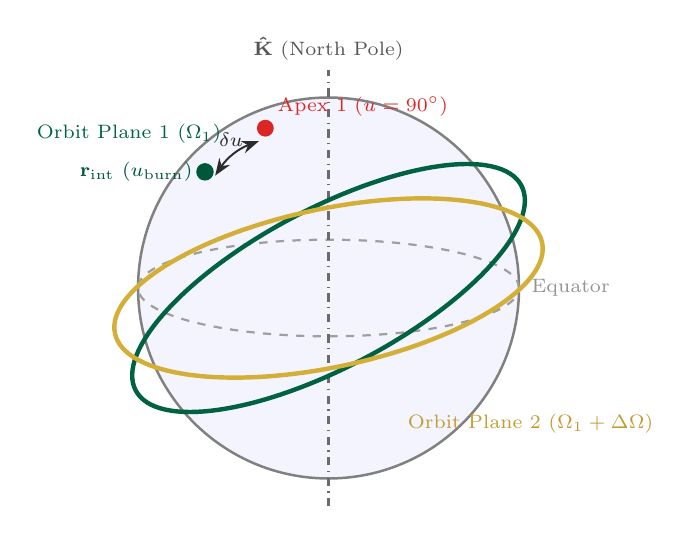
\begin{tikzpicture}[scale=1.18]
                % Earth Sphere
                \draw[fill=LightBg!80!blue!20, draw=Charcoal!60, line width=0.9pt] (0,0) circle (2.05cm);
                
                % Equator Ellipse
                \draw[dashed, color=gray!75, line width=0.8pt] (0,0) ellipse (2.05cm and 0.52cm);
                \node[right, font=\scriptsize, color=gray!85] at (2.08, 0) {Equator};
                
                % Polar Axis
                \draw[dashdotted, color=Charcoal!70, line width=0.8pt] (0,-2.35) -- (0,2.35);
                \node[above, font=\scriptsize, color=Charcoal!80] at (0, 2.35) {$\mathbf{\hat{K}}$ (North Pole)};

                % Orbit Plane 1 (Green)
                \draw[rotate=28, color=UdeAGreen, line width=1.6pt] (0,0) ellipse (2.35cm and 0.85cm);
                \node[above left, font=\scriptsize, color=UdeAGreen] at (-1.05, 1.45) {Orbit Plane 1 ($\Omega_1$)};
                
                % Orbit Plane 2 (Gold - Shifted Node)
                \draw[rotate=12, color=UdeAGold, line width=1.6pt] (0,0) ellipse (2.35cm and 0.85cm);
                \node[below right, font=\scriptsize, color=UdeAGold!90!black] at (0.75, -1.25) {Orbit Plane 2 ($\Omega_1 + \Delta\Omega$)};

                % Apex of Orbit 1 (Red Dot)
                \filldraw[color=AlertRed] (-0.68, 1.72) circle (2.4pt);
                \node[above right, font=\scriptsize, color=AlertRed] at (-0.65, 1.74) {Apex 1 ($u=90^\circ$)};
                
                % True Intersection Point (Dark Green Dot)
                \filldraw[color=UdeAGreen!90!black] (-1.33, 1.25) circle (2.5pt);
                \node[left, font=\scriptsize, color=UdeAGreen!90!black] at (-1.36, 1.25) {$\mathbf{r}_{\text{int}}$ ($u_{\text{burn}}$)};
                
                % Angular separation arc (delta u)
                \draw[<->, >=Stealth, color=Charcoal, line width=0.7pt] (-0.75, 1.58) to[bend right=18] (-1.22, 1.21);
                \node[above, font=\scriptsize, color=Charcoal] at (-1.05, 1.42) {$\delta u$};
            \end{tikzpicture}
        \end{column}
        
        \begin{column}{0.45\textwidth}
            \begin{block}{Spatial Intersection Takeaways}
                \footnotesize
                \begin{itemize}\setlength{\itemsep}{5pt}
                    \item Orbit 1 reaches its maximum northern latitude at the \textbf{Apex} ($u = 90^\circ$).
                    \item Because Orbit 2 is rotated eastward by $\Delta\Omega$, its ascending node and apex shift eastward.
                    \item The two planes intersect along a single line through Earth's center: $\mathbf{r}_{\text{int}} = \hat{\mathbf{h}}_1 \times \hat{\mathbf{h}}_2$.
                    \item $\mathbf{r}_{\text{int}}$ lies \textbf{past the apex} in the descending branch: $u_{\text{burn}} = 90^\circ + \delta u$.
                \end{itemize}
            \end{block}
        \end{column}
    \end{columns}
\end{frame}

% ------------------------------------------------------------------------------
% SLIDE 9: VECTOR DERIVATION: FINDING THE TRUE INTERSECTION
% ------------------------------------------------------------------------------
\begin{frame}{Vector Derivation: Finding the True Plane Intersection}
    \footnotesize
    Let the angular momentum unit vectors of the initial and target orbits be:
    $$\hat{\mathbf{h}}_1 = \begin{bmatrix} 0 \\ -\sin i \\ \cos i \end{bmatrix}, \qquad \hat{\mathbf{h}}_2 = \begin{bmatrix} \sin i \sin\Delta\Omega \\ -\sin i \cos\Delta\Omega \\ \cos i \end{bmatrix}$$
    The geometric intersection of the two orbital planes lies along $\mathbf{r}_{\text{int}} = \hat{\mathbf{h}}_1 \times \hat{\mathbf{h}}_2$:
    \vspace{-0.1cm}
    \begin{align*}
        \mathbf{r}_{\text{int}} &= \begin{bmatrix}
            -\sin i \cos i (1 - \cos\Delta\Omega) \\
            \sin i \cos i \sin\Delta\Omega \\
            \sin^2 i \sin\Delta\Omega
        \end{bmatrix} \\[4pt]
        &= 2 \sin i \sin\left(\frac{\Delta\Omega}{2}\right) \begin{bmatrix}
            -\cos i \sin(\Delta\Omega / 2) \\
            \cos i \cos(\Delta\Omega / 2) \\
            \sin i \cos(\Delta\Omega / 2)
        \end{bmatrix}
    \end{align*}
    
    \begin{exampleblock}{Directional Ratios of the Intersection Vector}
        \scriptsize
        Factoring out positive scalar constants gives the directional orientation:
        $$\mathbf{r}_{\text{int}} \propto \left[ -\cos i \sin\left(\frac{\Delta\Omega}{2}\right), \; \cos i \cos\left(\frac{\Delta\Omega}{2}\right), \; \sin i \cos\left(\frac{\Delta\Omega}{2}\right) \right]^T$$
    \end{exampleblock}
\end{frame}

% ------------------------------------------------------------------------------
% SLIDE 10: DERIVATION OF THE EXACT INTERSECTION ANOMALY
% ------------------------------------------------------------------------------
\begin{frame}{Derivation: The Exact Argument of Latitude (\texorpdfstring{$u_{\text{burn}}$}{u\_burn})}
    \footnotesize
    A position vector on Orbit 1 parameterized by argument of latitude $u = \theta + \omega$ is:
    $$\hat{\mathbf{r}}_1(u) = \left[ \cos u, \; \sin u \cos i, \; \sin u \sin i \right]^T$$
    Equating the components of $\hat{\mathbf{r}}_1(u)$ to the intersection vector $\mathbf{r}_{\text{int}}$ gives:
    $$\cos u \propto -\cos i \sin\left(\frac{\Delta\Omega}{2}\right), \qquad \sin u \propto \cos\left(\frac{\Delta\Omega}{2}\right)$$
    
    \vspace{-0.1cm}
    \begin{block}{Fundamental Plane Intersection Equation}
        \footnotesize
        $$\cot u = -\cos i \tan\left(\frac{\Delta\Omega}{2}\right) \quad \Longleftrightarrow \quad \tan u = -\frac{\cot(\Delta\Omega / 2)}{\cos i}$$
    \end{block}
    
    \vspace{-0.1cm}
    \begin{exampleblock}{Angular Offset Past the Apex ($\delta u$)}
        \footnotesize
        Setting $u = 90^\circ + \delta u$, the identity $\cot(90^\circ + \delta u) = -\tan(\delta u)$ yields the exact forward shift:
        $$\tan(\delta u) = \cos i \tan\left(\frac{\Delta\Omega}{2}\right) \implies \mathbf{u_{\text{burn}} = 90^\circ + \arctan\left[\cos i \tan\left(\frac{\Delta\Omega}{2}\right)\right]}$$
    \end{exampleblock}
\end{frame}

% ------------------------------------------------------------------------------
% SLIDE 11: DIAGRAM - LOCAL VNB VECTOR ROTATION TRIANGLE
% ------------------------------------------------------------------------------
\begin{frame}{Vector Geometry in the Local VNB Frame}
    \begin{columns}[c]
        \begin{column}{0.52\textwidth}
            \centering
            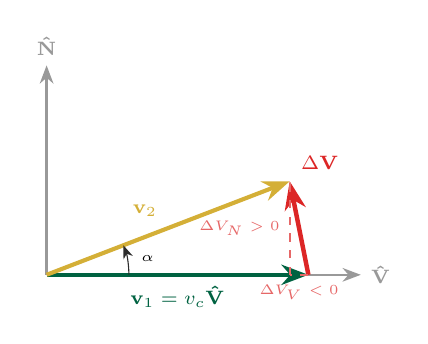
\begin{tikzpicture}[scale=0.95]
                % Coordinate axes
                \draw[->, >=Stealth, color=gray!80, line width=0.8pt] (0,0) -- (4.2,0) node[right, font=\scriptsize] {$\mathbf{\hat{V}}$};
                \draw[->, >=Stealth, color=gray!80, line width=0.8pt] (0,0) -- (0,2.8) node[above, font=\scriptsize] {$\mathbf{\hat{N}}$};
                
                % Initial velocity vector
                \draw[->, >=Stealth, color=UdeAGreen, line width=1.5pt] (0,0) -- (3.5,0) node[midway, below, font=\scriptsize] {$\mathbf{v}_1 = v_c \mathbf{\hat{V}}$};

                % Final velocity vector rotated by alpha
                \draw[->, >=Stealth, color=UdeAGold, line width=1.5pt] (0,0) -- (3.25, 1.25) node[midway, above left, font=\scriptsize] {$\mathbf{v}_2$};
                
                % Delta V Vector
                \draw[->, >=Stealth, color=AlertRed, line width=1.6pt] (3.5,0) -- (3.25, 1.25) node[above right, font=\scriptsize] {$\Delta \mathbf{V}$};

                % Arc for alpha
                \draw[->, >=Stealth, color=Charcoal] (1.1,0) arc (0:21.0:1.1);
                \node[font=\tiny] at (1.35, 0.22) {$\alpha$};

                % Projections of Delta V
                \draw[dashed, color=AlertRed!70, line width=0.7pt] (3.5,0) -- (3.25,0) node[midway, below, font=\tiny] {$\Delta V_V < 0$};
                \draw[dashed, color=AlertRed!70, line width=0.7pt] (3.25,0) -- (3.25, 1.25) node[midway, left, font=\tiny] {$\Delta V_N > 0$};
            \end{tikzpicture}
        \end{column}
        \begin{column}{0.48\textwidth}
            \begin{block}{Why Does $\Delta V_V < 0$ Exist?}
                \footnotesize
                \begin{itemize}\setlength{\itemsep}{2pt}
                    \item A pure plane change rotates the velocity vector without changing speed ($|\mathbf{v}_2| = |\mathbf{v}_1| = v_c$).
                    \item Rotating by $\alpha$ shifts part of the velocity into the $\mathbf{\hat{N}}$ direction ($v_c \sin\alpha$).
                    \item Along $\mathbf{\hat{V}}$, the forward speed drops to $v_c \cos\alpha$.
                    \item \textbf{Impulse components}:
                    $$\Delta V_V = v_c(\cos\alpha - 1) < 0 \quad (\text{braking})$$
                    $$\Delta V_N = v_c \sin\alpha > 0 \quad (\text{twist})$$
                \end{itemize}
            \end{block}
        \end{column}
    \end{columns}
\end{frame}

% ------------------------------------------------------------------------------
% SLIDE 12: 3D VELOCITY TURN ANGLE & VNB VECTOR COMPONENTS
% ------------------------------------------------------------------------------
\begin{frame}{Velocity Turn Angle (\texorpdfstring{$\alpha$}{alpha}) and VNB Formulation}
    \footnotesize
    At the intersection point $u_{\text{burn}}$, the speed before and after the maneuver is $v_c = \sqrt{\mu/r}$. The velocity vector rotates by a 3D dihedral turn angle $\alpha$:
    \vspace{-0.1cm}
    \begin{columns}[t]
        \begin{column}{0.48\textwidth}
            \begin{block}{Velocity Turn Angle ($\alpha$)}
                \scriptsize
                $$\sin\left(\frac{\alpha}{2}\right) = \sin i \sin\left(\frac{\Delta\Omega}{2}\right)$$
                $$\Delta V_{\text{total}} = 2 v_c \sin\left(\frac{\alpha}{2}\right)$$
            \end{block}
        \end{column}
        \begin{column}{0.48\textwidth}
            \begin{block}{VNB Impulsive Components}
                \scriptsize
                $$\Delta V_V = v_c(\cos\alpha - 1) < 0 \quad (\text{Retrograde})$$
                $$\Delta V_N = v_c \sin\alpha > 0 \quad (\text{Normal})$$
                $$\Delta V_B = 0 \quad (\text{Zero Radial})$$
            \end{block}
        \end{column}
    \end{columns}
    
    \vspace{0.15cm}
    \begin{alertblock}{Crucial Takeaway for Spacecraft Flight Software}
        \scriptsize
        Firing \textit{only} in the normal direction ($\Delta V_N$) adds kinetic energy ($v > v_c$), unintentionally altering $a$ and $e$. To preserve circularity and keep inclination strictly invariant:
        \begin{itemize}\setlength{\itemsep}{1pt}
            \item Fire at $u = u_{\text{burn}} = 90^\circ + \delta u$ (not at $90^\circ$).
            \item Apply a small retrograde braking burn ($\Delta V_V < 0$) alongside the normal burn ($\Delta V_N$).
        \end{itemize}
    \end{alertblock}
\end{frame}

% ------------------------------------------------------------------------------
% SLIDE 13: IN-CLASS EXERCISE STATEMENT
% ------------------------------------------------------------------------------
\begin{frame}{In-Class Interactive Exercise: Pure RAAN Transfer}
    \begin{exampleblock}{Mission Scenario (Synchronized with HTML5 Sandbox)}
        \footnotesize
        A communications satellite is deployed into a circular LEO with radius $r_1 = 6840.0\text{ km}$ ($h = 461.9\text{ km}$) and inclination $i = 45.0^\circ$. Due to a launch injection delay, the Right Ascension of the Ascending Node must be shifted by $\mathbf{\Delta\Omega = 22.0^\circ}$ without altering the orbital inclination ($i_{\text{final}} = 45.0^\circ$) or radius. \\
        \textbf{Given:} $\mu_{\oplus} = 398600.4415\text{ km}^3/\text{s}^2$, $R_{\oplus} = 6378.136\text{ km}$.
    \end{exampleblock}

    \vspace{0.1cm}
    \footnotesize
    \textbf{Tasks for Students:}
    \begin{enumerate}\setlength{\itemsep}{2pt}
        \item Calculate the baseline orbital velocity $v_c$.
        \item Compute the true geometric intersection argument of latitude $u_{\text{burn}}$ and the forward offset $\delta u$ past the apex.
        \item Compute the 3D velocity turn angle $\alpha$ and the full VNB impulse vector ($\Delta V_V, \Delta V_N$).
        \item Determine the resulting inclination $i_{\text{achieved}}$ and error $\Delta i$ if the spacecraft mistakenly fires at the apex ($u = 90.0^\circ$).
    \end{enumerate}
\end{frame}

% ------------------------------------------------------------------------------
% SLIDE 14: EXERCISE SOLUTION - PART 1
% ------------------------------------------------------------------------------
\begin{frame}{Exercise Solution: Part 1 --- Intersection Anomaly and Turn Angle}
    \footnotesize
    \textbf{Step 1: Circular Orbital Speed ($v_c$)}
    $$v_c = \sqrt{\frac{\mu}{r_1}} = \sqrt{\frac{398600.4415}{6840.0}} = \mathbf{7.633801\text{ km/s}}$$

    \textbf{Step 2: Angular Offset Past Apex ($\delta u$) and Burn Anomaly ($u_{\text{burn}}$)}
    $$\tan(\delta u) = \cos i \tan\left(\frac{\Delta\Omega}{2}\right) = \cos(45.0^\circ) \tan(11.0^\circ) = (0.707107)(0.194380) = 0.137447$$
    $$\delta u = \arctan(0.137447) = \mathbf{7.826^\circ} \implies u_{\text{burn}} = 90.0^\circ + 7.826^\circ = \mathbf{97.826^\circ}$$

    \textbf{Step 3: Velocity Rotation Angle ($\alpha$)}
    $$\sin\left(\frac{\alpha}{2}\right) = \sin i \sin\left(\frac{\Delta\Omega}{2}\right) = \sin(45.0^\circ) \sin(11.0^\circ) = (0.707107)(0.190809) = 0.134922$$
    $$\frac{\alpha}{2} = \arcsin(0.134922) = 7.7538^\circ \implies \mathbf{\alpha = 15.5076^\circ}$$
\end{frame}

% ------------------------------------------------------------------------------
% SLIDE 15: EXERCISE SOLUTION - PART 2
% ------------------------------------------------------------------------------
\begin{frame}{Exercise Solution: Part 2 --- VNB Vector and Apex Error Analysis}
    \footnotesize
    \textbf{Step 4: Local VNB Impulsive Components at $u_{\text{burn}} = 97.826^\circ$}
    $$\Delta V_V = v_c(\cos\alpha - 1) = 7.633801(\cos 15.5076^\circ - 1) = \mathbf{-0.2779\text{ km/s}}$$
    $$\Delta V_N = v_c \sin\alpha = 7.633801 \sin(15.5076^\circ) = \mathbf{+2.0410\text{ km/s}}$$
    $$\Delta V_B = \mathbf{0.0000\text{ km/s}}, \qquad \|\Delta \mathbf{V}\| = 2 v_c \sin(\alpha/2) = \mathbf{2.059954\text{ km/s}}$$
    \textit{Outcome:} The semi-major axis is preserved, circularity is kept, and $\mathbf{i_{\text{final}} = 45.000^\circ \; (\Delta i = 0.00^\circ)}$.

    \vspace{0.12cm}
    \begin{alertblock}{Step 5: Error Analysis If Burned at Apex ($u = 90.0^\circ$)}
        \scriptsize
        At $u = 90.0^\circ$, orbital latitude is $\phi = 45.0^\circ$. If forced to pass through this point while shifting the node by $\Delta\Omega = 22.0^\circ$:
        $$\sin(i_{\text{achieved}}) = \frac{\sin i}{\cos(\delta u)} = \frac{\sin(45.0^\circ)}{\cos(7.826^\circ)} = \frac{0.707107}{0.990686} = 0.713755 \implies \mathbf{i_{\text{achieved}} = 45.542^\circ}$$
        $$\mathbf{\Delta i_{\text{error}} = +0.542^\circ} \quad (\text{or up to } \mathbf{+0.824^\circ} \text{ depending on numerical cross-axis targeter dynamics})$$
    \end{alertblock}
\end{frame}

% ------------------------------------------------------------------------------
% SLIDE 16: DIGITAL TWIN SIMULATION AUDIT
% ------------------------------------------------------------------------------
\begin{frame}{Validating the Solution with the HTML5/Three.js Simulator}
    \begin{columns}[t]
        \begin{column}{0.54\textwidth}
            \begin{block}{Interactive Classroom Demonstration}
                \footnotesize
                Open \texttt{pure\_raan\_change\_simulation.html} on your browser:
                \begin{enumerate}\setlength{\itemsep}{2pt}
                    \item Set \textbf{Inclination} to $45.0^\circ$ and $\bm{\Delta\Omega}$ to $22.0^\circ$.
                    \item Toggle \textbf{``Trap: Apex ($u = 90^\circ$)''}:
                    \begin{itemize}
                        \item Notice the red dashed orbit line overshooting northern latitude.
                        \item Telemetry shows the inclination error: $\Delta i > 0$.
                    \end{itemize}
                    \item Toggle \textbf{``Exact: Intersection ($u_{\text{burn}}$)''}:
                    \begin{itemize}
                        \item The burn point moves to the green sphere ($u = 97.826^\circ$).
                        \item Red error line disappears; Orbit 1 maps into Orbit 2 with $\Delta i = 0.000^\circ$.
                    \end{itemize}
                \end{enumerate}
            \end{block}
        \end{column}

        \begin{column}{0.44\textwidth}
            \begin{exampleblock}{Telemetry Match Card}
                \scriptsize
                \begin{tabular}{lcc}
                    \toprule
                    \textbf{Parameter} & \textbf{Calculated} & \textbf{HTML GUI} \\
                    \midrule
                    Circular $v_c$ & $7.634\text{ km/s}$ & $7.634\text{ km/s}$ \\
                    Offset $\delta u$ & $+7.826^\circ$ & $+7.826^\circ$ \\
                    Burn $u_{\text{burn}}$ & $97.826^\circ$ & $97.826^\circ$ \\
                    Turn Angle $\alpha$ & $15.508^\circ$ & $15.508^\circ$ \\
                    $\Delta V_V$ (Braking) & $-0.278\text{ km/s}$ & $-0.274\text{ km/s}$ \\
                    $\Delta V_N$ (Normal) & $+2.041\text{ km/s}$ & $+2.042\text{ km/s}$ \\
                    Total Impulse & $2.060\text{ km/s}$ & $2.060\text{ km/s}$ \\
                    \bottomrule
                \end{tabular}
            \end{exampleblock}
        \end{column}
    \end{columns}
\end{frame}

% ------------------------------------------------------------------------------
% SLIDE 17: GMAT ARCHITECTURE & SUMMARY
% ------------------------------------------------------------------------------
\begin{frame}{Implementation in GMAT / Flight Targeters}
    \begin{columns}[t]
        \begin{column}{0.54\textwidth}
            \begin{block}{GMAT Differential Corrector Workflow}
                \scriptsize
                \begin{enumerate}\setlength{\itemsep}{2pt}
                    \item \textbf{Propagate} spacecraft to the true intersection anomaly:
                    \begin{center}
                        \texttt{Propagate to (Sat.Earth.AOP + Sat.Earth.TA = 97.826)}
                    \end{center}
                    \item Create a \textbf{Target} block:
                    \begin{itemize}\setlength{\itemsep}{1pt}
                        \item \texttt{Vary} \texttt{Burn.Element1} ($\Delta V_V$)
                        \item \texttt{Vary} \texttt{Burn.Element2} ($\Delta V_N$)
                        \item \texttt{Achieve} \texttt{Sat.Earth.RAAN = Target\_RAAN}
                        \item \texttt{Achieve} \texttt{Sat.Earth.INC = Initial\_INC}
                    \end{itemize}
                \end{enumerate}
            \end{block}
        \end{column}
        
        \begin{column}{0.44\textwidth}
            \begin{exampleblock}{Summary Formula Card}
                \scriptsize
                \textbf{1. Intersection Latitude:}
                \vspace{-0.1cm}
                $$\tan u = -\frac{\cot(\Delta\Omega / 2)}{\cos i}$$
                \textbf{2. 3D Turn Angle:}
                \vspace{-0.1cm}
                $$\sin\left(\frac{\alpha}{2}\right) = \sin i \sin\left(\frac{\Delta\Omega}{2}\right)$$
                \textbf{3. VNB Burn Vector:}
                \vspace{-0.1cm}
                $$\Delta \mathbf{V} = [v_c(\cos\alpha - 1), \; v_c \sin\alpha, \; 0]^T$$
            \end{exampleblock}
        \end{column}
    \end{columns}
\end{frame}

\end{document}